

\section{Influence Probability Analysis}
\label{sec:influenceanalysis}

Using the four static models discussed above, we built an influence graph with anti-virus engines on \vt\ and analyzed 
the influence probability ($p_{u,v}$) between each pair of engines.

\noindent{\underline{\textit{Methodology.}}}
We implement our analysis using several stages of map, filter, and reduce in Spark~\cite{spark}. 
We filter out engines taking fewer than 20000 actions,
since engines taking too few actions cannot produce meaningful results.
There are 59 engines left,
and the average number of actions taken by these engines is around 392K.
For confidentiality reasons, we omit vendors' name in the following discussion
and use numbers from 0 to 58 to represent these vendors.


\noindent{\underline{\textit{Analysis results and implications.}}}
For each static model, 
we construct an influence table with calculated influence probability values ($p_{u,v}$), 
with $u$ as row number and $v$ as column number.
We visualize these influence tables with heat maps in Figure~\ref{fig:heat}. 
Each $cell(u, v)$ represents the relative heat color of $p_{u,v}$, 
and red means more influence from $u$ to $v$. 

We also sum all $p_{u,v}$ values in a column in each influence table 
to calculate trustworthiness of engine $v$ using Equation~\ref{eq:trust}. 
Table~\ref{tab:trust} lists the maximum, minimum, and average trustworthiness values of all the engines under four different models.
The results can serve as a quantitative measurement for how trustworthy anti-virus engines are. 

In all the four heat maps, there are two columns with almost all cells in red,
which means that these vendors influenced by all other vendors and are less trustworthy.
On the other hand, quite a few vendors are not influenced by any vendors (blue columns).
This result suggests that most vendors perform predictions on their own and thus can be trusted. 
However, our result should also ring an alarm to online malware detection service users and security experts that 
we cannot treat all engines with the same level of trust 
and the results from some of them should be at least examined more closely if not discarded.

At the same time, there are several rows with many cells in red, especially in the last two heat map, 
which means that there are vendors which influence many vendors,
where there are a set of vendors that do not influence other vendors (blue rows).
Different from the effect of columns which shows the trustworthiness of a vendor by users, 
the effect of rows is related to how vendors view (and trust) each other. 
Certain vendors are highly regarded by many other vendors so that 
their decision results are often referenced by other vendors.

Interestingly, the vendors that are heavily influenced by others are not the ones that influence others, 
suggesting that the vendors with lower trustworthiness by users are also not trusted by other vendors. 

\begin{table}[h!]
\centering
\footnotesize
{
\begin{tabular}{l|l|l|l}
\hline
Model                & Max     & Min & Average \\
\hline                            
%\cline{1-1}
{\bf Bernoulli}                    & 108.78   & 0.04 & 5.40 \\
{\bf Jaccard Index}                & 118.20   & 0.05 & 6.15 \\
{\bf Bernoulli with Partial Credit} & 3545.34  & 1.63 & 138.45 \\
{\bf Jaccard Index with Partial Credit} & 4177.98 & 2.02 & 155.18 \\
\hline
\end{tabular}
}
\caption{Trustworthiness. 
%\footnotesize{
(Maximum, minimum, and average trustworthiness values under four different models.)
%}
}
\label{tab:trust}
\end{table}


%Finally, we observe that although the four static models show similar trends of influence relationship 
%and the relative rankings of engines in terms of influence are similar,
%their absolute influence probability values differ. 
%Bernoulli distribution and Jaccard index have influence probability values
%that are about 30 to 40 times higher than
%Bernoulli and Jaccard index with partial credit. 
%This shows that {\color{red} influence is shared among vendors take actions earlier than others. I have no idea what sentense means. if you cannot explain well, just remove this sentence.}.

{\bf Observation 1:} 
{\em Certain anti-virus vendors are influenced by almost all other vendors in their malware detection decisions and are less trustworthy, 
while quite a few trustworthy vendors have influence on many other vendors.}

\section{Influence Probability Prediction}
\label{sec:predict}

The analysis results of vendor influence above are encouraging.
With these results, we take a step further and ask 
{\em if it is possible to predict whether or not an engine's prediction of 
a file submission should be trusted (i.e., not influenced by other engines)?}
We now discuss the prediction model we built to answer this question.

\noindent{\underline{\textit{Methodology.}}}
We first split all the \pe\ submissions we collected into a training set and a testing set based on 
the SHA256 values of the submitted files. 
We place all submissions with SHA256 values starting with a numeric character, 
i.e., from `0' to `9', into training set
and all the rest (starting from `a' to `f') into the testing set.
We use Spark to implement both the training and the testing process.
%Similar to our training stage process, 
%we first reduce all submissions based on submitted files,
%next filter out files without action propagation, 
%and then sort submissions chronologically. 


%\noindent{\underline{\textit{Training stage methodology.}}}
During the training stage, we use the training set to build an influence graph and
learn $p_{u,v}$ of each edge in the graph using the four static models discussed in Section~\ref{sec:influenceprob}.
The calculation of $p_{u,v}$ is the same as in Section~\ref{sec:influenceanalysis}.

%\noindent{\underline{\textit{Testing stage methodology.}}}
During the prediction stage, for each submission in the testing set, 
we predict whether or not an engine $v$ will take an action $a$ following other engines 
if it has not taken that action yet. 
%Specifically, we use a tunable threshold $\theta$
%and predict $v$ will follow its neighbors to take the action $a$ in the future
%if $p_v(S_v(a))>\theta$.
Specifically, to test a submission, we first use Equation~\ref{eq:setp} to
calculate $p_v(S_v(a))$, the probability that $v$ will follow its neighbors to take the same action, 
for all engines that have labeled the submitted file only as benign in their history. 
These engines are of interest to us because positive influence, 
the type of influence in this study, only happens 
when an engine changes its prediction decision from benign to malware.

We then compare $p_v(S_v(a))$ with a {\em tunable threshold $\theta$} to predict whether $v$ will label the file as malware (if $p_v(S_v(a))>\theta$) or not.
Next, we compare this prediction with the actual action that $v$ took in the testing set to deduct true positives (TPs) where both our prediction 
and the actual fact label the submission as malware, 
false negatives (FNs) where our prediction labels the submission as benign and the actual labeling is malware. 
Thus, TP means our prediction is the same as the fact 
and both show the engine changes its labeling from benign to malware, an indication that the decision 
of this engine on the submission is in deed affected by other engines.
Similarly, we can obtain false positives (FPs) 
and true negatives (TNs).
%After processing all submissions for a file, 
%we calculate $p_v(S_v(a))$ for all engines  
%that label the file as benign but have not labeled the file as malware.
%We compare $p_v(S_v(a))$ with $\theta$ to count false positives (FPs) and true negatives (TNs).
In the final stage, we calculate the overall TP, TN, FP, and FN rates for all different files.

\begin{figure}[t!]
\begin{center}
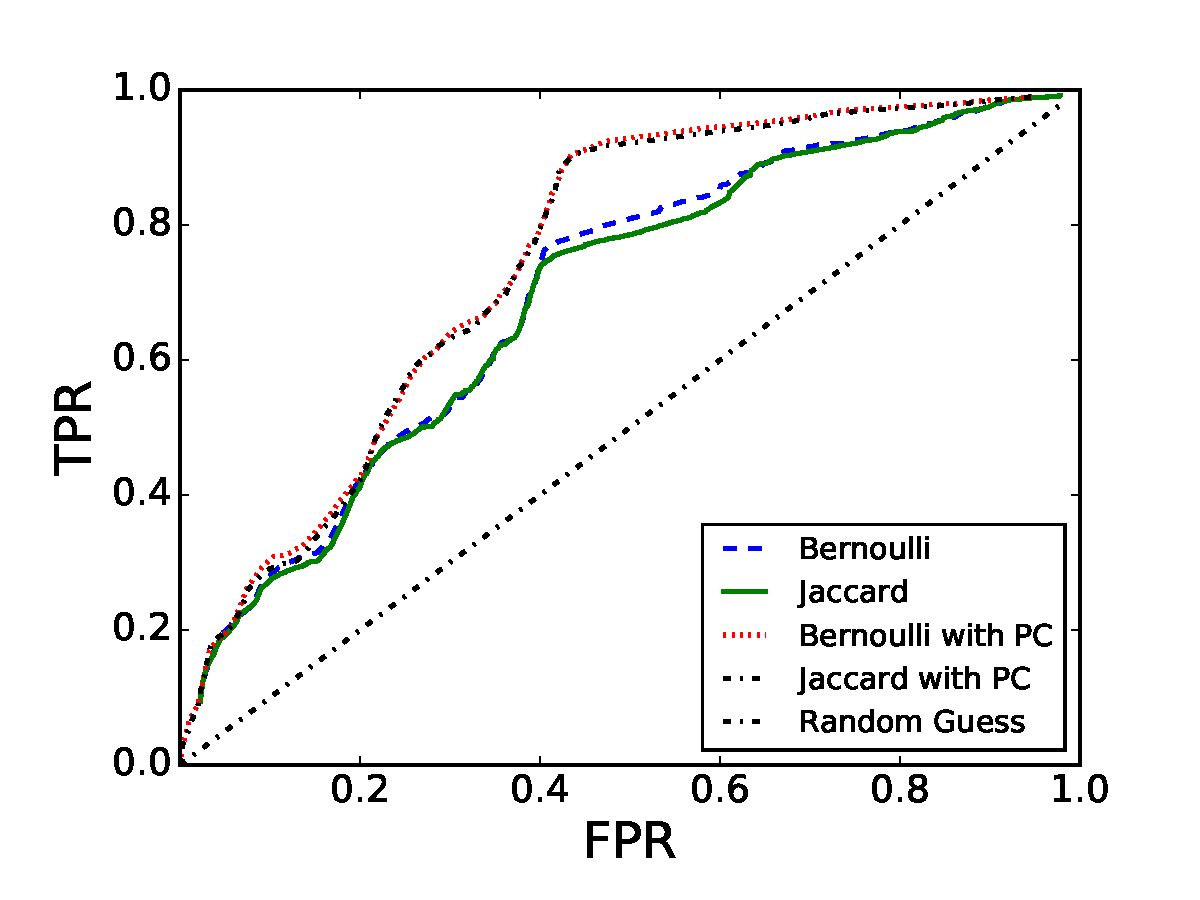
\includegraphics[width=2in]{figure/predict}
\vspace{-0.1in}
\caption{ROC comparisons of Static Models. 
(How true positive rate (TPR) changes with false positive rate (FPR). 
We change probability threshold from 0.1\% to 99.9\% with step 0.1\%. 
We compute TPR and FPR for each probability threshold to draw the curve.)
}
\label{fig:predict}
\end{center}
\vspace{-0.1in}
\end{figure}

\noindent{\underline{\textit{Prediction results.}}}
We change the threshold $\theta$ from 0.1\% to 99.9\% 
and measure the accuracy of the four static models using ROC (Receiver Operating Characteristic) curves,
with true positive rate ($TPR = TP/(TP+FN)$) as X-axis
and false positive rate ($FPR = FP/(FP + FN)$) as Y-axis. 
Figure~\ref{fig:predict} plots the ROC curves for the four static models.
A larger area under the ROC curve means higher accuracy.
We compare our prediction models with random guess, 
which is represented by the diagonal line between (0,0) to (1,1) in the figure. 

We find that all models are more accurate than random guess
and using partial credits improves the accuracy of both Bernoulli and Jaccard index.
This result is encouraging;
even with a simple prediction model like ours, we can already obtain satisfactory prediction accuracy of whether an engine's decision has been influenced by others.

{\bf Observation 2:} 
{\em Our influence prediction model can accurately predict whether or not an anti-virus engine's labeling of a submission should be trusted. }




